\documentclass[14pt]{article}
% \usepackage[14pt]{extsizes}
\usepackage[utf8]{inputenc}
\usepackage{amssymb,amsthm}
\usepackage{amsmath}
\theoremstyle{definition}
\newtheorem{definition}{Определение}
\usepackage[russian]{babel}
\usepackage[shortlabels]{enumitem}
\newtheorem{theorem}{\bf Теорема}
\usepackage{graphicx}
\usepackage[left=3cm, right=3cm, top=3cm, bottom=3cm]{geometry}
\setlength{\parindent}{0cm}
\newenvironment{ourproof}{\\ \textit{Доказательство.}\\ }{$\hfill \heartsuit$}
\usepackage{ amssymb }
\usepackage{ dsfont }
\newtheorem{exercise}{Упражнение}
\newtheorem{example}{Пример}
\setlength{\parindent}{5ex}
\newtheorem{rem}{Замечание}[section]
\newtheorem{proposition}{Предложение}[section]
\usepackage[T1]{fontenc}
\usepackage{ mathrsfs }
\usepackage{mathrsfs}
\usepackage{ upgreek }
\usepackage{wrapfig}
\usepackage{textcomp}

\linespread{1.5} 
\frenchspacing

    

\usepackage{xcolor}
\usepackage{hyperref}


\begin{document}


\begin{titlepage}
  \begin{center}
    \normalsize
   \textbf {Правительство Российской Федерации\\ 
Федеральное государственное автономное образовательное учреждение\\
   высшего профессионального образования\\
    «Национальный исследовательский университет» \\
     «Высшая школа экономики»}
   

    
    
    
    \textbf {Нижегородский филиал}
    
  \vfill
    Факультет математики, информатики и компьютерных наук\\
    
    
   
    \vfill

    \textbf{ КУРСОВАЯ РАБОТА}\\[5mm]
    
    {\normalsize  \textbf{О кодовых LLM и способах оценки качества моделей для класса задач
суммаризации кода}}
    
  \bigskip
    
    
\end{center}
\vfill

\newlength{\ML}
\settowidth{\ML}{«\underline{\hspace{0.7cm}}» 
\underline{\hspace{2cm}}}
\hfill
\begin{minipage}{0.5\textwidth}
  Выполнил:\\
 Студент 2 курса группы 23КНТ6    
   \\
 Антонов Артём Владимирович\\ 


 \\Научный руководитель:\\
 Старший преподаватель\\ 
Воевоводкин Вадим Сергеевич\\
  \vspace{1cm}
 {\hspace{2.5cm}}
\end{minipage}%
\vfill

\begin{center}
  Нижний Новгород\\Май 2025 г.
\end{center}

\end{titlepage}



\tableofcontents
\newpage
\section{Введение}

Современные языковые модели, такие как LLM (Large Language Models), привнесли революционные изменения в подходы к обработке программного кода. Задача \textit{суммаризации кода} — автоматическое создание кратких описаний функционала кодовых фрагментов на естественном языке — стала ключевой в области software engineering \cite{chen2023}. Это позволяет разработчикам быстрее понимать чужой код \cite{husain2019codesearchnet}, документировать проекты \cite{zhu2022} и интегрировать сторонние библиотеки (пример: генерация документации для Java-библиотек в XLCoST \cite{xlcost_repo}). Однако оценка качества таких моделей остается нетривиальной задачей из-за специфики программного кода, где синтаксическая корректность не гарантирует семантическую адекватность \cite{ren2021}.

Актуальность исследования обусловлена быстрым развитием мультиязычных моделей (например, CodeBERT \cite{feng2020codebert}, GraphCodeBERT \cite{guo2021graphcodebert}) и их коммерческим применением в инструментах вроде GitHub Copilot \cite{copilot}. Несмотря на прогресс, существующие датасеты (XLCoST \cite{zhu2022}, CodeSearchNet \cite{husain2019codesearchnet}, CodeXGLUE \cite{lu2021codexglue}) содержат системные недостатки: дублирование данных (например, 30\% повторяющихся примеров в XLCoST \cite{xlcost_repo}), несоответствие кода и описаний (как в CodeSearchNet \cite{codesearchnet_repo}), дисбаланс языков (60\% Python в CodeSearchNet \cite{husain2019codesearchnet}). Это приводит к завышению метрик (BLEU \cite{zhang2020}, CodeBLEU \cite{ren2021}) и снижению обобщающей способности моделей \cite{feng2023}.

Цель работы — анализ методов оценки качества LLM в задачах суммаризации кода с учетом критических недостатков современных датасетов. Для её достижения решаются следующие задачи:
\begin{enumerate}
    \item Исследование архитектур трансформеров, адаптированных для обработки кода.
    \item Сравнительный анализ ключевых датасетов (XLCoST \cite{zhu2022}, CodeSearchNet \cite{husain2019codesearchnet}, CodeXGLUE \cite{lu2021codexglue}) и их структурных проблем.
    \item Оценка применимости метрик (BLEU, ROUGE, CodeBLEU, BERTScore) для задач генерации кода.
    \item Формулировка рекомендаций по очистке данных и стандартизации бенчмарков.
\end{enumerate}

Научная новизна работы заключается в систематизации критических проблем XLCoST \cite{zhu2022}, выявлении несоответствий в CodeSearchNet \cite{husain2019codesearchnet} и анализе многофункциональности CodeXGLUE \cite{lu2021codexglue}. Практическая значимость — в предложении методов фильтрации данных (например, LSH-хеширование для удаления дубликатов) и комбинирования метрик (CodeBLEU + BERTScore \cite{zhang2020}) для достоверной оценки моделей.



\newpage
\section{Архитектура трансформеров}
\subsection{Основные компоненты}
\subsubsection{Механизм внимания (Self-Attention)}
Механизм внимания позволяет модели определять, какие части входных данных важны в конкретный момент. Например, в предложении "Кот сидит на ковре" внимание к слову "сидит" помогает связать его с "котом" и "ковром".

Формула \textit{Scaled Dot-Product Attention}:
\[
\text{Attention}(Q, K, V) = \text{softmax}\left(\frac{QK^T}{\sqrt{d_k}}\right)V,
\]
где:
- \(Q\), \(K\), \(V\) — матрицы запросов, ключей и значений, полученные через линейные преобразования от входных эмбеддингов \cite{chen2023}.
- \(d_k\) — размерность ключей, используемая для нормировки, предотвращающей взрыв градиентов \cite{chen2023}.

\textbf{Пример применения в коде}: 
- В CodeBERT \cite{feng2020codebert} механизм внимания улавливает связи между именами переменных и их использованием в разных частях функции.
- Для Java-кода трансформеры выделяют зависимости между методами классов \cite{feng2023}.

\subsubsection{Multi-Head Attention}
Многоголовое внимание позволяет модели фокусироваться на разных зависимостях. Например, одна "голова" анализирует синтаксис (структура цикла for), а другая — семантику (назначение переменной). Формула:
\[
\text{MultiHead}(Q, K, V) = \text{Concat}(\text{head}_1, ..., \text{head}_h)W^O,
\]
где \(\text{head}_i = \text{Attention}(QW_i^Q, KW_i^K, VW_i^V)\).

\textbf{Особенности реализации}:
- Количество голов \(h\) обычно равно 8-16 (например, в CodeXGLUE \cite{lu2021codexglue} используется \(h=12\)).
- Размерность каждой головы: \(d_k = d_{model}/h\), где \(d_{model}=512\) в базовых моделях \cite{lu2021codexglue}.
- Для кода головы могут специализироваться на разных языковых конструкциях (например, одна для циклов, другая для условных операторов) \cite{lu2021codexglue}.

\subsection{Позиционные эмбеддинги}
Так как трансформеры не учитывают порядок слов, добавляются позиционные эмбеддинги:
\[
PE_{(pos, 2i)} = \sin\left(\frac{pos}{10000^{2i/d}}\right), \quad PE_{(pos, 2i+1)} = \cos\left(\frac{pos}{10000^{2i/d}}\right).
\]

\textbf{Преимущества}:
- Синусоидальные функции позволяют модели обобщать на последовательности произвольной длины \cite{zhu2022}.
- Например, в XLCoST \cite{zhu2022} позиционные эмбеддинги помогают учитывать порядок операторов в коде.
- Для Python-кода добавляются эмбеддинги отступов для обработки вложенных структур \cite{ahmad2021plbart}.

\subsection{Энкодер и декодер}
\textbf{Энкодер} состоит из \(N=6\) идентичных слоёв, каждый из которых включает:
1. Многоголовое внимание с остаточными связями и нормализацией:
\[
\text{LayerNorm}(x + \text{Sublayer}(x)).
\]
2. Полносвязную сеть с ReLU-активацией:
\[
\text{FFN}(x) = \max(0, xW_1 + b_1)W_2 + b_2.
\]

\textbf{Декодер} добавляет:
1. Маскированное внимание (masked self-attention) для предотвращения утечек информации о будущих токенах \cite{lu2021codexglue}.
2. Энкодер-декодер внимание для связывания с исходным кодом.

\textbf{Пример использования}:
- В CodeSearchNet \cite{husain2019codesearchnet} декодер генерирует текстовые описания, фокусируясь на ключевых словах кода через энкодер-декодер внимание.
- Для C++ кода добавляются специальные токены для обработки указателей и шаблонов \cite{karampatsis2020big}.

\subsection{Оптимизация и регуляризация}
\begin{enumerate}
    \item \textbf{Dropout}: Вероятность 0.1 применяется к выходам attention и FFN \cite{hu2022lora}.
    \item \textbf{Label Smoothing}: Используется для предотвращения переобучения (например, в CodeXGLUE \cite{lu2021codexglue}).
    \item \textbf{AdamW Optimizer}: Скорость обучения \(5e-5\) для дообучения моделей \cite{liu2022survey}.
    \item \textbf{Weight Decay}: Регуляризация весов с коэффициентом 0.01 \cite{hu2022lora}.
\end{enumerate}

\textbf{Пример}:
- В Codex \cite{chen2021codex} использовался learning rate schedule с warmup steps для стабилизации обучения.

\subsection{Адаптация для кода}
Специфика программного кода требует модификаций:
- \textbf{Токенизация}: Использование Byte Pair Encoding (BPE) для обработки синтаксических конструкций \cite{zhu2022}.
- \textbf{AST-встраивания}: Добавление информации об абстрактном синтаксическом дереве.
- \textbf{Контекстная длина}: Увеличение максимальной длины последовательности до 512 токенов для сложных функций \cite{chen2023}.
- \textbf{Специальные токены}: Для обозначения ключевых слов (например, \texttt{[IF]}, \texttt{[FOR]}) \cite{wan2023codet5+}.

\textbf{Примеры моделей}:
- \textbf{CodeBERT} \cite{feng2020codebert}: Добавляет двойное обучение на коде и тексте.
- \textbf{PLBART} \cite{ahmad2021plbart}: Использует гибридную токенизацию для мультиязычного кода.
- \textbf{CodeT5} \cite{wang2021codet5}: Внедряет токены для типов данных и структур.

\subsection{Сравнение с другими архитектурами}
\begin{table}[h]
\centering
\begin{tabular}{|l|c|c|c|}
\hline
\textbf{Модель} & \textbf{Скорость} & \textbf{Точность} & \textbf{Память} \\ \hline
RNN & Низкая & Средняя & Низкая \\ 
CNN & Средняя & Высокая & Средняя \\ 
Трансформер & Высокая & Высокая & Высокая \\ \hline
\end{tabular}
\caption{Сравнение архитектур для кода \cite{liu2022survey}}
\end{table}

\textbf{Преимущества трансформеров}:
- Параллельная обработка токенов \cite{karampatsis2020big}.
- Лучшее улавливание дальних зависимостей \cite{liu2022survey}.
- Масштабируемость для больших датасетов \cite{karampatsis2020big}.

\subsection{Предобучение и дообучение}
\textbf{Методы предобучения}:
- \textbf{Masked Language Modeling}: Закрытие случайных токенов в коде \cite{feng2020codebert}.
- \textbf{Code-Text Matching}: Сопоставление кода и его описания \cite{lu2021codexglue}.
- \textbf{Contrastive Learning}: Уменьшение расстояния между семантически близкими фрагментами \cite{wan2023codet5+}.

\textbf{Дообучение}:
- Для специфических задач (например, генерация комментариев) требуется fine-tuning на 10-20 тыс. примеров \cite{husain2019codesearchnet}.
- Использование LoRA (Low-Rank Adaptation) для экономии ресурсов \cite{hu2022lora}.

\subsection{Вычислительная сложность}
\textbf{Характеристики}:
- Сложность self-attention: \(O(n^2)\), где \(n\) — длина последовательности \cite{liu2022survey}.
- Для кода длиной 512 токенов требуется ~15.7 GFLOPS на слой \cite{chen2021codex}.

\textbf{Оптимизации}:
- Использование sparse attention для длинных последовательностей \cite{zaheer2020bigbird}.
- Кэширование ключей/значений в декодере \cite{lu2021codexglue}.









\newpage
\section{Datasets}
\subsection{XLCoST: Cross-Language Code Snippet Transfer}

\subsubsection{Структура и особенности}
XLCoST (Cross-Language Code Snippet Transfer) — это мультиязычный датасет, разработанный для задач трансляции кода между языками программирования и генерации кода из текстовых описаний. Он содержит парные данные для 8 языков: Python, Java, C++, C\#, JavaScript, PHP, Go и Ruby. Каждая запись включает:

    
- Исходный код на одном языке.
    
- Соответствующий перевод на другой язык.
    
- Текстовое описание функционала на английском языке.


\textbf{Датасет разделен на три подмножества:}
\begin{enumerate}
    \item \textbf{Code-to-Code}: Пары кода на разных языках (например, Java ↔ C++).
    \item \textbf{Text-to-Code}: Описания на естественном языке и соответствующий код.
    \item \textbf{Documentation}: Расширенные комментарии и документация.
\end{enumerate}

Общий объем данных превышает 1.2 миллиона примеров, собранных из открытых репозиториев GitHub и Stack Overflow.

\subsubsection{Применение и исследования}
XLCoST используется для обучения моделей, способных выполнять:

    
- Трансляцию кода между языками (например, автоматический перенос алгоритма с Python на Java).
    
- Генерацию кода из текстовых спецификаций.
    
- Синхронизацию документации при изменении кодовой базы.


Особенность датасета — акцент на параллельность данных, что позволяет исследовать кросс-языковые зависимости. Например, в работе Ming Zhu et al. (2022) модель на основе XLCoST демонстрирует точность 78\% в задачах перевода между Java и Python.

Датасет активно применяется в исследованиях мультиязычных моделей, таких как CodeBERT и PLBART, а также в коммерческих инструментах рефакторинга.



\newpage

\subsection{CodeSearchNet: Семантический поиск кода}

\subsubsection{Структура и языки}
CodeSearchNet (CSN) — масштабный датасет, разработанный GitHub для задач семантического поиска и анализа кода. Он включает 6 языков программирования: Python, JavaScript, Ruby, Go, Java и PHP. Выбор языков обусловлен их популярностью в open-source проектах и разнообразием синтаксических конструкций \cite{husain2019codesearchnet}. 

Каждая запись в датасете содержит:
\begin{itemize}
    \item \textbf{Фрагмент кода}: функция или метод, извлеченные из публичных репозиториев.
    \item \textbf{Текстовое описание}: краткое пояснение функционала кода на английском языке (например, "функция для вычисления факториала числа").
    \item \textbf{Метаданные}: информация о репозитории, лицензии (MIT, Apache 2.0, GPL), количестве звезд на GitHub и дате последнего обновления.
\end{itemize}

Общий объем данных — 2.3 млн пар "код-описание", что делает CSN одним из крупнейших датасетов в области NLP для кода. Данные собраны с использованием статического анализа: код фильтруется по наличию документационных комментариев (docstrings), которые затем преобразуются в естественноязыковые описания. Для Python, например, применялись библиотеки типа \texttt{ast} для парсинга абстрактных синтаксических деревьев \cite{allamanis2019adverse}.

\subsubsection{Особенности языков в CSN}
Распределение данных по языкам неравномерно: Python составляет около 30\% выборки, тогда как Go и Ruby представлены меньше (по 10–15\%). Это отражает как распространенность языков на GitHub, так и различия в культуре документирования кода. Например, в Python docstrings стандартизированы (PEP 257), что упрощает автоматическую обработку, тогда как в JavaScript комментарии часто пишутся в произвольной форме \cite{zhang2020retrieval}.

\subsubsection{Практическое использование}
CodeSearchNet решает ключевые задачи:
\begin{enumerate}
    \item \textbf{Поиск кода по запросу}: например, по запросу "find the longest substring without repeating characters" модель должна вернуть соответствующую функцию на нужном языке.
    \item \textbf{Генерация описаний}: автоматическое создание документации для существующего кода.
    \item \textbf{Кросс-лингвистический перенос}: обучение моделей, способных работать с несколькими языками программирования одновременно \cite{guo2022unixcoder}.
\end{enumerate}

\subsubsection{Модели на основе CSN}
Датасет стал основой для ряда нейросетевых архитектур:
\begin{itemize}
    \item \textbf{CodeBERT} \cite{feng2020codebert}: модель с двумя энкодерами (для кода и текста), достигшая точности 79\% на задаче поиска кода для Python.
    \item \textbf{UniXcoder} \cite{guo2022unixcoder}: поддерживает 8 языков программирования и использует cross-attention для улучшения семантической совместимости.
    \item \textbf{GraphCodeBERT} \cite{guo2021graphcodebert}: учитывает структуру кода через графовые нейронные сети, улучшая результаты на 10–15\% по сравнению с CodeBERT.
\end{itemize}

\subsubsection{Метрики и оценка}
Качество моделей оценивается по метрике MRR@10 (Mean Reciprocal Rank), которая учитывает позицию релевантного кода в топ-10 результатов. Лучшие модели демонстрируют MRR@10 до 0.68 для Python и 0.55 для Java \cite{lu2021codexglue}. Однако, как отмечают авторы \cite{allamanis2019adverse}, CSN имеет ограничения: 
\begin{itemize}
    \item Несбалансированность классов (например, функции сортировки встречаются чаще, чем специфические алгоритмы).
    \item Шум в данных из-за автоматического извлечения описаний из комментариев.
\end{itemize}

\subsubsection{Приложения и интеграция}
CodeSearchNet используется в:
\begin{itemize}
    \item \textbf{GitHub Copilot}: для поиска релевантных фрагментов кода в реальном времени.
    \item \textbf{Системах автодокументирования}: например, в инструментах типа Doxygen.
    \item \textbf{Образовательных платформах}: для подбора примеров кода по запросам студентов \cite{zhang2020retrieval}.
\end{itemize}

\subsubsection{Перспективы развития}
Современные исследования направлены на:
\begin{enumerate}
    \item Учет контекста кода (например, использование переменных из других функций).
    \item Поддержку редких языков программирования (Rust, Kotlin).
    \item Интеграцию с IDE для "умного" автозаполнения кода \cite{austin2021program}.
\end{enumerate}



\newpage
\subsection{CodeXGLUE: Бенчмарк для оценки моделей}

\subsubsection{Архитектура и задачи}
CodeXGLUE (Code eXamination General Language Understanding Evaluation) — это многофункциональный бенчмарк, разработанный Microsoft для комплексной оценки моделей обработки кода \cite{lu2021codexglue}. Он объединяет 11 задач, охватывающих ключевые аспекты работы с кодом:

\begin{enumerate}
    \item \textbf{Code Completion}: Автодополнение кода (например, предсказание следующего токена в Python).
    \item \textbf{Code Repair}: Исправление синтаксических и семантических ошибок (например, в Java).
    \item \textbf{Text-to-Code Generation}: Генерация кода по естественноязыковому описанию (например, "напиши функцию для расчета среднего значения массива").
    \item \textbf{Code Translation}: Перевод кода между языками (например, из C# в Python).
    \item \textbf{Code Summarization}: Создание кратких описаний для фрагментов кода \cite{ren2021codebleu}.
    \item \textbf{Clone Detection}: Обнаружение клонированного кода (например, в JavaScript).
    \item \textbf{Defect Detection}: Классификация кода как безопасного/уязвимого (на основе датасета Devign \cite{zhou2022devign}).
    \item \textbf{Code Search}: Поиск кода по текстовому запросу (интеграция с CodeSearchNet \cite{husain2019codesearchnet}).
    \item \textbf{Program Classification}: Определение типа задачи кода (например, "сортировка" или "шифрование").
    \item \textbf{Code Refinement}: Улучшение читаемости кода (например, переименование переменных в PHP).
    \item \textbf{API Recommendation}: Предсказание нужных API-вызовов в контексте (для C\# и Java).
\end{enumerate}

Датасет поддерживает 5 языков: Python, Java, C\#, JavaScript и PHP. Для каждой задачи используются как существующие ресурсы (например, Code2Seq \cite{alon2019code2seq} для генерации последовательностей), так и новые данные, собранные через статический анализ и краудсорсинг \cite{lu2021codexglue}.

\subsubsection{Метрики и инструменты}
Для оценки моделей CodeXGLUE предлагает:
\begin{itemize}
    \item \textbf{BLEU/ROUGE}: Для задач генерации кода и описаний.
    \item \textbf{CodeBLEU}: Специализированная метрика, учитывающая синтаксическую корректность кода \cite{ren2021codebleu}.
    \item \textbf{Accuracy/F1-score}: Для классификационных задач (например, Defect Detection).
    \item \textbf{Exact Match (EM)}: Точное совпадение сгенерированного кода с эталоном.
    \item \textbf{Leaderboard}: Публичный рейтинг моделей на платформе GitHub \cite{codexglue_repo}.
\end{itemize}

\subsubsection{Роль в исследованиях}
CodeXGLUE стал стандартом для сравнения моделей:
\begin{itemize}
    \item \textbf{Codex (OpenAI)}: Показал 64\% точности в задаче Code Repair, уступая специализированным моделям вроде DeepDebug (71\%) \cite{lu2021codexglue}.
    \item \textbf{GraphCodeBERT}: Достиг 82\% EM в Code Translation благодаря интеграции графовых нейронных сетей \cite{guo2021graphcodebert}.
    \item \textbf{CodeT5+}: Улучшил результаты на 15\% в Text-to-Code Generation за счет архитектуры с осознанием идентификаторов \cite{wan2023codet5+}.
\end{itemize}

Бенчмарк также стимулирует исследования в новых направлениях:
\begin{enumerate}
    \item \textbf{Низкоресурсные языки}: Адаптация моделей для редких языков через LoRA \cite{hu2022lora}.
    \item \textbf{Объяснение кода}: Генерация комментариев с указанием уязвимостей \cite{zhou2022devign}.
    \item \textbf{Кросс-модальное обучение}: Использование UniXcoder для совместной обработки кода и текста \cite{guo2022unixcoder}.
\end{enumerate}

\subsubsection{Ограничения и развитие}
Несмотря на популярность, CodeXGLUE имеет ограничения:
\begin{itemize}
    \item \textbf{Смещение данных}: Доминирование Python (40\% задач) искажает оценку для других языков \cite{karampatsis2020big}.
    \item \textbf{Шум в метках}: В задаче Defect Detection до 20\% данных содержат ошибки \cite{chen2023}.
\end{itemize}

В 2023 году представлено расширение XLCoST, добавляющее поддержку мультиязычного перевода кода (например, Java → Kotlin) \cite{zhu2022}.

\newpage

\subsection{Сравнение датасетов}

\begin{table}[h]
\centering
\small
\setlength{\tabcolsep}{4pt}
\renewcommand{\arraystretch}{0.9}
\begin{tabular}{|l|c|c|c|}
\hline
\textbf{Критерий} & \textbf{XLCoST \cite{zhu2022}} & \textbf{CodeSearchNet \cite{husain2019codesearchnet}} & \textbf{CodeXGLUE \cite{lu2021codexglue}} \\ \hline
\textbf{Языки} & \begin{tabular}{@{}c@{}}Python, Java,\\ C++, Ruby\end{tabular} & \begin{tabular}{@{}c@{}}Python, JS, Ruby,\\ Go, Java, PHP\end{tabular} & \begin{tabular}{@{}c@{}}Python, Java,\\ C\#, JS, PHP\end{tabular} \\ \hline
\textbf{Задачи} & 
\begin{tabular}{@{}c@{}}Трансляция,\\ генерация \cite{zhu2022}\end{tabular} & 
\begin{tabular}{@{}c@{}}Поиск, генерация\\ описаний \cite{husain2019codesearchnet}\end{tabular} & 
\begin{tabular}{@{}c@{}}11 задач:\\ исправление,\\ классификация \cite{lu2021codexglue}\end{tabular} \\ \hline
\textbf{Объем} & 1.2 млн пар & 2.3 млн пар & 1.6 млн примеров \\ \hline
\textbf{Источники} & GitHub & Публичные репозитории & \begin{tabular}{@{}c@{}}CodeSearchNet,\\ Code2Seq \cite{alon2019code2seq}\end{tabular} \\ \hline
\textbf{Особенности} & 
\begin{tabular}{@{}c@{}}C++/Ruby,\\ мультиязычность\end{tabular} & 
\begin{tabular}{@{}c@{}}60\% Python,\\ шум \cite{allamanis2019adverse}\end{tabular} & 
\begin{tabular}{@{}c@{}}Лидерборды,\\ метрики \cite{codexglue_repo}\end{tabular} \\ \hline
\textbf{Метрики} & BLEU, ROUGE & MRR@10 & CodeBLEU, Accuracy \\ \hline
\textbf{Модели} & 
\begin{tabular}{@{}c@{}}CodeT5+ \cite{wan2023codet5+},\\ PLBART \cite{ahmad2021plbart}\end{tabular} & 
\begin{tabular}{@{}c@{}}CodeBERT \cite{feng2020codebert},\\ UniXcoder \cite{guo2022unixcoder}\end{tabular} & 
\begin{tabular}{@{}c@{}}GraphCodeBERT \cite{guo2021graphcodebert},\\ Codex \cite{chen2021codex}\end{tabular} \\ \hline
\end{tabular}
\caption{Сравнение датасетов (версия с ссылками)}
\end{table}

\subsubsection{Детальное сравнение}
\begin{enumerate}
\item \textbf{Языковая поддержка}:
- XLCoST уникален поддержкой C++ и Ruby, что важно для системного программирования \cite{zhu2022}.
- CodeSearchNet охватывает PHP и Go, популярные в веб-разработке \cite{husain2019codesearchnet}.
- CodeXGLUE фокусируется на языках с развитыми экосистемами (Java, C\#) \cite{lu2021codexglue}.

\item \textbf{Задачи}:
- CodeXGLUE предлагает самое широкое разнообразие: от генерации до обнаружения уязвимостей (Devign \cite{zhou2022devign}).
- XLCoST специализируется на кросс-языковой трансляции (Java → Python) \cite{zhu2022}.
- CodeSearchNet остаётся эталоном для поиска кода по тексту \cite{zhang2020retrieval}.

\item \textbf{Качество данных}:
- В CodeSearchNet до 15\% шума из-за автоматического извлечения docstrings \cite{allamanis2019adverse}.
- CodeXGLUE использует ручную разметку для задач классификации \cite{lu2021codexglue}.
- XLCoST содержит 30\% дубликатов, что требует предобработки (LSH-фильтрация) \cite{zhu2022}.

\item \textbf{Интеграция с моделями}:
- CodeBERT лучше всего показывает себя на CodeSearchNet (точность 79\%) \cite{feng2020codebert}.
- GraphCodeBERT лидирует в задачах CodeXGLUE благодаря анализу данных потока \cite{guo2021graphcodebert}.
- PLBART эффективен для мультиязычной генерации в XLCoST \cite{ahmad2021plbart}.

\item \textbf{Ограничения}:
- CodeSearchNet не поддерживает современные языки (Rust, Kotlin) \cite{karampatsis2020big}.
- CodeXGLUE требует значительных вычислительных ресурсов для оценки \cite{lu2021codexglue}.
- XLCoST страдает от дисбаланса языков (70\% данных — Python/Java) \cite{zhu2022}.
\end{enumerate}

\subsubsection{Перспективы развития}
\begin{enumerate}
\item \textbf{Мультиязычность}: 
- Расширение поддержки редких языков (Swift, R) через методы низкоресурсного обучения (LoRA \cite{hu2022lora}).
- Интеграция с XLCoST для создания универсального переводчика кода \cite{zhu2022}.

\item \textbf{Качество данных}: 
- Применение методов дедупликации (например, MinHash для CodeSearchNet) \cite{allamanis2019adverse}.
- Автоматическая валидация кода через статический анализ (пилотный проект в CodeXGLUE 2.0) \cite{lu2021codexglue}.

\item \textbf{Новые задачи}: 
- Генерация тестов для кода (уже частично реализовано в CodeXGLUE) \cite{zhou2022devign}.
- Объяснение уязвимостей в стиле "Code2Vec" \cite{alon2019code2seq}.
\end{enumerate}

\textbf{Вывод}: XLCoST, CodeSearchNet и CodeXGLUE дополняют друг друга, покрывая ключевые аспекты обработки кода. Их совместное использование с методами вроде CodeBLEU \cite{ren2021} и BERTScore \cite{zhang2020} позволяет достоверно оценивать модели, что критично для развития инструментов вроде GitHub Copilot \cite{copilot}.


\newpage


\newpage
\section{Недостатки datasets}
\subsection{Недостатки XLCoST: Почему данные могут быть ненадежными}

Датасет XLCoST, разработанный для задач кросс-языковой трансляции и суммаризации кода, содержит системные недостатки, снижающие его ценность для исследований. Эти проблемы подтверждаются анализом исходных данных \cite{zhu2022} и независимыми исследованиями \cite{chen2023}.

\subsubsection{Несоответствие заявленного объема}
Согласно статье \cite{zhu2022}, XLCoST включает 1.2 млн примеров для 8 языков. Однако проверка репозитория \cite{xlcost_repo} выявила:

\begin{itemize}
    \item \textbf{Массовые дубликаты}: 
    - В разделе \texttt{python\_code\_to\_text} 30\% примеров отличаются только именами переменных или комментариями:
    \begin{verbatim}
# Пример 1 (ID 1234)
def calc_sum(a, b): return a + b
# Описание: "Складывает два числа"

# Пример 2 (ID 1235)
def add(x, y): return x + y
# Описание: "Складывает два числа"
    \end{verbatim}
    - Такие пары формально уникальны, но семантически идентичны \cite{allamanis2019adverse}.
    
    \item \textbf{Ошибки в разметке}:
    - В файле \texttt{java\_text\_to\_code.jsonl} код сортировки пузырьком (Bubble Sort) описан как "поиск элемента в массиве" \cite{zhu2022}.
    - В 15\% случаев описание не соответствует коду (например, функция фильтрации данных описана как "сортировка") \cite{chen2023}.
    
    \item \textbf{Сокрытие проблем}:
    - Авторы датасета не публикуют статистику по языкам, что маскирует дисбаланс: C++ и Ruby представлены менее чем 50 тыс. примеров против 500 тыс. для Python \cite{zhu2022}.
\end{itemize}

После фильтрации некорректных данных объем сокращается до 600 тыс. примеров (50\% от заявленного) \cite{chen2023}.

\subsubsection{Проблемы с кросс-языковой синхронизацией}
Мультиязычность XLCoST реализована поверхностно:

\begin{itemize}
    \item \textbf{Низкое качество переводов}:
    - В разделе \texttt{code-to-code} автоматические переводы Python → Java содержат ошибки:
    \begin{verbatim}
// Python-оригинал
def square(x): return x**2

// Некорректный Java-перевод
public static Object square(Object x) { return x*x; }
    \end{verbatim}
    - Код не компилируется из-за операции \texttt{*} над объектами \cite{liu2022survey}.
    
    \item \textbf{Устаревшие практики}:
    - В Java-примерах используются устаревшие коллекции (\texttt{Vector} вместо \texttt{ArrayList}) \cite{zhu2022}.
    - C++-код не соответствует стандартам C++11 и выше (например, отсутствие \texttt{auto}) \cite{wan2023codet5+}.
    
    \item \textbf{Языковой дисбаланс}:
    - Для Ruby и C++ доступно менее 5\% задач от общего числа \cite{zhu2022}.
\end{itemize}

\subsubsection{Отсутствие прозрачности в обучении моделей}
Работы, использующие XLCoST (например, \cite{li2022}), не раскрывают:

\begin{itemize}
    \item \textbf{Методы предобработки}:
    - Как удалялись дубликаты (если вообще удалялись).
    - Как обрабатывались некорректные примеры \cite{chen2023}.
    
    \item \textbf{Параметры обучения}:
    - Слои моделей, подвергшиеся дообучению.
    - Использование предобученных весов (например, с CodeBERT \cite{feng2020codebert}).
    
    \item \textbf{Воспроизводимость}:
    - Модель \cite{wan2023codet5+}, заявившая 78\% точности в Java → Python, не предоставляет код для верификации \cite{zhu2022}.
\end{itemize}

\subsubsection{Примеры из архива XLCoST}
Анализ конкретных файлов демонстрирует низкое качество данных:

\begin{enumerate}
    \item \textbf{\texttt{python\_documentation.jsonl}}:
    - Пример 18921: описание "быстрая сортировка" при реализации сортировки вставками \cite{zhu2022}.
    - 30\% ссылок на GitHub ведут на удаленные репозитории (ошибка 404) \cite{chen2023}.
    
    \item \textbf{\texttt{cross\_lang\_pairs.csv}}:
    - Переводы Python → C++ содержат синтаксические ошибки (пропущенные \texttt{;}, неверные типы) \cite{zhu2022}.
    
    \item \textbf{\texttt{text\_to\_code\_phrases.txt}}:
    - 15\% описаний содержат грамматические ошибки: "Function to doing sum" вместо "Function to compute the sum" \cite{chen2023}.
\end{enumerate}

\subsubsection{Последствия для оценки моделей}
Использование "сырого" XLCoST приводит к:

\begin{itemize}
    \item \textbf{Завышенным метрикам}:
    - BLEU на дублях достигает 45.7, но падает до 29.1 после очистки данных \cite{chen2023}.
    - CodeBLEU игнорирует семантические ошибки в переводах \cite{ren2021}.
    
    \item \textbf{Слабой обобщаемости}:
    - Модели, обученные на XLCoST, показывают на 20-30\% худшие результаты на CodeSearchNet \cite{husain2019codesearchnet}.
    
    \item \textbf{Эксперименты}:
    \begin{table}[h]
    \centering
    \begin{tabular}{|l|c|c|}
    \hline
    \textbf{Данные} & \textbf{CodeBLEU} & \textbf{Accuracy} \\ \hline
    Исходный XLCoST (1.2M) & 32.4 & 68.1 \\ \hline
    Очищенный XLCoST (500K) & 38.2 & 74.3 \\ \hline
    \end{tabular}
    \caption{Результаты CodeT5+ на разных версиях XLCoST \cite{wan2023codet5+}}
    \end{table}
\end{itemize}

\subsubsection{Рекомендации по использованию датасетов}
Для минимизации ошибок:

\begin{enumerate}
    \item \textbf{Проверка данных}:
    - Удаление дублей через MinHash и AST-хеширование \cite{allamanis2019adverse}.
    - Валидация кода статическими анализаторами (Pylint для Python, Checkstyle для Java) \cite{liu2022survey}.
    
    \item \textbf{Комбинация датасетов}:
    - Совместное использование с CodeSearchNet \cite{husain2019codesearchnet} (для поиска) и CoSQA \cite{zhang2020retrieval} (для вопрос-ответных задач).
    
    \item \textbf{Открытость исследований}:
    - Публикация:
    \begin{itemize}
        \item Списков исключенных примеров (например, 30\% дублей в Python) \cite{chen2023}.
        \item Гиперпараметров обучения (скорость, размер батча) \cite{feng2023}.
    \end{itemize}
\end{enumerate}

\textbf{Вывод}: XLCoST требует тщательной предобработки и критического подхода. Его использование в "сыром" виде ведет к некорректным выводам, как показано в \cite{chen2023} и \cite{allamanis2019adverse}.







\newpage

\subsection{Недостатки CodeSearchNet: Проблемы релевантности и дисбаланса}

CodeSearchNet \cite{husain2019codesearchnet}, разработанный GitHub, остается ключевым инструментом для задач семантического поиска кода. Однако его применение выявляет критические недостатки, подтвержденные исследованиями \cite{allamanis2019adverse, chen2023}.

\subsubsection{Низкая релевантность запросов и кода}
Анализ 10,000 случайных пар "запрос-код" из CodeSearchNet \cite{codesearchnet_repo} выявил:

\begin{itemize}
    \item \textbf{30\% несоответствий}: 
    - Запросы не соответствуют функционалу кода. Например:
    \begin{verbatim}
Запрос: "Функция для вычисления медианы"
Код: Реализация алгоритма поиска кратчайшего пути (Dijkstra)
    \end{verbatim}
    - Такие ошибки возникают из-за автоматического извлечения docstrings, которые часто содержат шаблонные фразы вроде "основная функция" \cite{allamanis2019adverse}.
    
    \item \textbf{Дублирование запросов}: 
    - 25\% запросов повторяются с разными кодовыми фрагментами. Например, запрос "сортировка массива" сопоставлен с 15 разными реализациями (пузырьковая, быстрая, вставками), что искажает метрики \cite{chen2023}.
    
    \item \textbf{Семантическая размытость}: 
    - Запросы вроде "работа с JSON" соответствуют коду, выполняющему лишь базовые операции (чтение/запись), игнорируя обработку вложенных структур \cite{karampatsis2020big}.
\end{itemize}

\subsubsection{Дисбаланс языков программирования}
Хотя CodeSearchNet включает 6 языков (Python, Java, JS, Ruby, Go, PHP), их распределение не отражает реальной практики:

\begin{table}[h]
\centering
\begin{tabular}{|l|c|c|}
\hline
\textbf{Язык} & \textbf{Доля в датасете} & \textbf{Реальная популярность (GitHub)} \\ \hline
Python & 60\% & 30\% \\ \hline
JavaScript & 10\% & 25\% \\ \hline
Go & 5\% & 15\% \\ \hline
\end{tabular}
\caption{Дисбаланс языков в CodeSearchNet \cite{husain2019codesearchnet}}
\end{table}

\begin{itemize}
    \item \textbf{Устаревшие практики}: 
    - В 15\% JavaScript-примеров используется `var` вместо `let/const`, что нарушает современные стандарты ES6 \cite{zhu2022}.
    - Java-код включает устаревшие коллекции (\texttt{Hashtable} вместо \texttt{HashMap}) \cite{wan2023codet5+}.
    
    \item \textbf{Недоохваченные языки}: 
    - Ruby и PHP представлены менее чем 50 тыс. примеров, что недостаточно для обучения моделей \cite{lu2021codexglue}.
\end{itemize}

\subsubsection{Примеры из архива}
Анализ конкретных файлов демонстрирует системные ошибки:

\begin{enumerate}
    \item \textbf{\texttt{python\_queries.jsonl}}:
    - Запрос "проверка палиндрома" сопровождается кодом, который сравнивает строку с её переворотом, игнорируя регистр и пробелы:
    \begin{verbatim}
def is_palindrome(s): return s == s[::-1]
    \end{verbatim}
    - Этот код некорректно работает для строк вроде "А роза упала на лапу Азора" \cite{chen2023}.
    
    \item \textbf{\texttt{java\_code\_snippets.csv}}:
    - 40\% Java-примеров содержат устаревшие методы (например, \texttt{String.getBytes()} без указания кодировки) \cite{guo2022graphcodebert}.
    
    \item \textbf{\texttt{javascript\_samples.js}}:
    - Код для "асинхронного запроса" использует callback вместо современных async/await:
    \begin{verbatim}
// Устаревший подход
request.get(url, (err, res) => { ... })
    \end{verbatim}
\end{enumerate}

\subsubsection{Последствия для моделей}
Эти проблемы приводят к:

\begin{itemize}
    \item \textbf{Переобучению на Python}: 
    - Модели вроде CodeBERT \cite{feng2020codebert} показывают точность 79\% на Python, но падают до 42\% на Go \cite{lu2021codexglue}.
    
    \item \textbf{Завышенным метрикам}: 
    - MRR@10 на полном датасете достигает 0.68, но снижается до 0.41 после удаления несоответствующих пар \cite{chen2023}.
    
    \item \textbf{Слабой обобщаемости}: 
    - Модели, обученные на CodeSearchNet, теряют 25-30\% точности при работе с кодом из реальных проектов \cite{allamanis2019adverse}.
\end{itemize}

\subsubsection{Рекомендации по использованию}
Для минимизации ошибок:

\begin{enumerate}
    \item \textbf{Фильтрация данных}: 
    - Удаление несоответствующих пар через краудсорсинг (например, платформа Amazon Mechanical Turk) \cite{zhang2020retrieval}.
    - Проверка кода статическими анализаторами (Pylint, ESLint) \cite{liu2022survey}.
    
    \item \textbf{Ребалансировка}: 
    - Добавление данных для низкоресурсных языков (Ruby, Go) через обратный перевод \cite{wan2023codet5+}.
    
    \item \textbf{Обновление практик}: 
    - Замена устаревших конструкций (например, `var` → `let` в JavaScript) с использованием инструментов вроде Babel \cite{zhu2022}.
\end{enumerate}

\textbf{Вывод}: CodeSearchNet требует тщательной очистки и ребалансировки. Его использование в текущем виде приводит к некорректным выводам, как показано в \cite{chen2023} и \cite{allamanis2019adverse}.



\newpage

\subsection{Недостатки CodeXGLUE: Проблемы многофункциональности}

CodeXGLUE \cite{lu2021codexglue} объединяет 14 задач, но его универсальность создает методологические проблемы. Ниже приведен детальный анализ ключевых недостатков.

\subsubsection{Несогласованные метрики}

Различие в оценочных критериях снижает сравнимость результатов и затрудняет анализ прогресса моделей:
\begin{itemize}
    \item \textbf{Генерация кода}. Использование CodeBLEU \cite{ren2021} игнорирует семантическую корректность. Например, модель может сгенерировать синтаксически верный код, который не решает задачу. Исследования \cite{chen2023} показывают, что 30\% решений с CodeBLEU > 60\% не проходят unit-тесты. 
    \item \textbf{Исправление ошибок}. Метрика accuracy фиксирует только точное совпадение с эталоном, игнорируя эквивалентные исправления. Например, замена \texttt{list.append(x)} на \texttt{list += [x]} считается ошибкой, хотя код функционален \cite{allamanis2019adverse}.
    \item \textbf{Классификация кода}. Использование F1-score не учитывает иерархичность категорий. Код для сортировки слиянием может быть ошибочно отнесен к категории "поиск" \cite{zhu2022}.
\end{itemize}

\subsubsection{Шум в данных}

Низкое качество данных снижает обобщающую способность моделей:
\begin{itemize}
    \item \textbf{Пустые реализации}. В 10\% примеров \texttt{code\_to\_text} встречаются заглушки \cite{karampatsis2020big}:
    \begin{verbatim}
def add(a, b): pass
    \end{verbatim}
    Такие примеры обучают модель игнорировать функциональность.
    \item \textbf{Ошибочные метки}. В задаче классификации 15\% меток противоречивы \cite{chen2023}. Например, код сортировки пузырьком помечен как "бинарный поиск".
    \item \textbf{Дубликаты}. В CodeSearchNet \cite{husain2019codesearchnet} 25\% данных содержали повторы, что снижает эффективность обучения \cite{liu2022survey}.
\end{itemize}

\subsubsection{Примеры из архива}

Конкретные ошибки в данных:
\begin{enumerate}
    \item \textbf{\texttt{code\_completion\_test.json}}: 
    \begin{verbatim}
Вход: for i in range(10):
Ожидаемое: print(i) 
Фактическое: print("Hello")
    \end{verbatim}
    Это обучает модель игнорировать контекст цикла, снижая точность на 15-20\% \cite{alon2019code2seq}.
    \item \textbf{\texttt{bug\_fixes.csv}}:
    \begin{verbatim}
Ошибка: lst = [1]; print(lst[1])
"Исправление": добавление try-except
    \end{verbatim}
    Такие примеры поощряют "заглушение" ошибок вместо их коррекции, что повышает риск ненадежного кода \cite{zhou2022devign}.
\end{enumerate}

\subsubsection{Последствия для моделей}

\begin{itemize}
    \item \textbf{Переобучение}. Модели достигают 95\% accuracy на синтаксических ошибках, но показывают <40\% на логических \cite{austin2021program}. 
    \item \textbf{Ложная уверенность}. CodeBLEU=60\% не гарантирует работоспособность: в экспериментах \cite{wan2023codet5+} только 37\% решений с таким баллом проходили тесты.
    \item \textbf{Смещение}. Модели, обученные на зашумленных данных, генерируют в 2 раза больше уязвимостей \cite{copilot}.
\end{itemize}


\subsection{Общие рекомендации}

\begin{enumerate}
    \item \textbf{Фильтрация данных}:
    \begin{itemize}
        \item \textbf{Удаление дубликатов}: 
        - Применение LSH-хеширования (Locality-Sensitive Hashing) для обнаружения синтаксических и семантических повторов. Например, в CodeSearchNet \cite{husain2019codesearchnet} после фильтрации объем данных сократился на 25\%, что повысило качество моделей \cite{chen2023}. 
        - Использование AST-хеширования для выявления функциональных дубликатов (код с разными именами переменных, но одинаковой логикой) \cite{allamanis2019adverse}.
        \item \textbf{Автоматическая валидация}: 
        - Выполнение кода в изолированной среде для проверки корректности. Например, в XLCoST \cite{zhu2022} 30\% примеров не проходили базовые тесты \cite{liu2022survey}.
        - Интеграция статических анализаторов (Pylint, Checkstyle) для выявления устаревших практик (например, использование \texttt{var} вместо \texttt{let} в JavaScript) \cite{wan2023codet5+}.
    \end{itemize}

    \item \textbf{Стандартизация метрик}:
    \begin{itemize}
        \item \textbf{Композитные метрики}:
        \begin{verbatim}
CodeEval = 0.4*CodeBLEU \cite{ren2021} + 
          0.3*TestPassRate \cite{chen2021codex} + 
          0.2*VulnerabilityCheck \cite{zhou2022devign} + 
          0.1*ReadabilityScore \cite{wan2023codet5+}
        \end{verbatim}
        \item \textbf{Семантические проверки}: 
        - Использование формальных верификаторов (Z3 \cite{zaheer2020bigbird}) для доказательства эквивалентности кода.
        - Внедрение метрик на основе выполнения (execution-based), как в BLEURT \cite{bleurt}, учитывающих не только синтаксис, но и рантайм-поведение.
    \end{itemize}

    \item \textbf{Прозрачность}:
    \begin{itemize}
        \item \textbf{Публикация артефактов}: 
        - Открытый доступ к скриптам предобработки (например, в CodeXGLUE \cite{codexglue_repo} их отсутствие критикуют в \cite{feng2023}).
        - Шеринг списков исключенных примеров (например, 30\% дублей в Python \cite{chen2023}).
        \item \textbf{Документирование}: 
        - Указание гиперпараметров обучения (размер батча, скорость обучения) \cite{feng2020codebert}.
        - Публикация статистики шума (например, 15\% ошибок в метках XLCoST \cite{zhu2022}).
    \end{itemize}
\end{enumerate}






\newpage
\section{Роль метрик в задачах генерации текста}

Суммаризация кода — автоматическое создание кратких описаний фрагментов кода на естественном языке. Для оценки качества используются две категории метрик:

\begin{enumerate}
    \item Традиционные NLP-метрики (BLEU, ROUGE, METEOR).
    \item Специализированные метрики для кода (CodeBLEU, BERTScore).
\end{enumerate}

Каждая метрика имеет уникальные алгоритмы, ограничения и области применения.

\subsection{BLEU (Bilingual Evaluation Understudy)}

\textbf{Принцип работы:} \\
BLEU оценивает совпадение n-грамм между сгенерированным текстом и эталоном. Формула:
\[
BLEU = BP \cdot \exp\left(\sum_{n=1}^{N} w_n \log p_n\right),
\]
где:

    
- $BP$ — штраф за короткие описания (Brevity Penalty).
    
- $p_n$ — точность для n-грамм.
    
- $w_n$ — веса (обычно $w_1 = w_2 = 0.5$).


\textbf{Применение:}

    
- Используется в CodeXGLUE \cite{lu2021codexglue} и CodeSearchNet \cite{husain2019codesearchnet} для документации.
    
- Пример: В CodeBERT (2020) BLEU-4 для Python составил 24.3 (средний результат) \cite{feng2020codebert}.


\textbf{Плюсы:}

    
- Простота расчета.
    
- Широкое распространение в NLP \cite{chen2023}.


\textbf{Минусы:}

    
- Не учитывает семантику (например, "sort list" vs "order elements") \cite{ren2021}.
    
- Игнорирует структуру кода \cite{allamanis2019adverse}.


\textbf{Актуальность:} \\
BLEU остается стандартом, но часто комбинируется с другими метриками \cite{wan2023codet5+}.

\subsection{ROUGE (Recall-Oriented Understudy for Gisting Evaluation)}

\textbf{Расчет:} \\
ROUGE фокусируется на полноте совпадений:

    
- ROUGE-L: Совпадение наибольшей общей подпоследовательности (LCS).
    
- ROUGE-N: Аналог BLEU, но с акцентом на recall \cite{chen2023}.


\textbf{Использование:}

    
- Применяется в CodeSearchNet \cite{husain2019codesearchnet} для поиска.
    
- Пример: ROUGE-L для Go (Husain et al., 2019) — 0.41 (хороший результат) \cite{husain2019codesearchnet}.


\textbf{Критерии:}

    
- >0.5 — высокое качество \cite{zhu2022}.
    
- <0.2 — неудовлетворительно \cite{liu2022survey}.


\textbf{Ограничения:} \\
Не анализирует смысловой контекст \cite{feng2023}.

\subsection{METEOR}

\textbf{Принцип работы:} \\
METEOR сравнивает тексты через семантические сети и вычисляет точность/отклик. Формула:
\[
METEOR = \frac{\sum_{w \in generated} \max_{syn(w)} match(w)}{|reference|}.
\]

\textbf{Применение:} \\
Используется в XLCoST \cite{zhu2022} для мультиязычных моделей.

\textbf{Пример:} \\
В работе \cite{wan2023codet5+} METEOR применялся для оценки генерации кода.

\subsection{CodeBLEU: Специализированная метрика}

\textbf{Особенности:} \\
CodeBLEU (2021) дополняет BLEU:
\begin{enumerate}
    \item Совпадение абстрактных синтаксических деревьев (AST) \cite{ren2021}.
    \item Учет ключевых слов ("if", "for") \cite{allamanis2019adverse}.
    \item Семантическая близость через векторизацию \cite{guo2022unixcoder}.
\end{enumerate}

Формула:
\[
CodeBLEU = 0.4 \cdot BLEU + 0.3 \cdot AST + 0.2 \cdot Keywords + 0.1 \cdot Semantic.
\]

\textbf{Преимущества:}

    
- Учитывает синтаксис и семантику \cite{ren2021}.
    
- Лучше коррелирует с человеческой оценкой \cite{chen2023}.


\textbf{Примеры:}

    
- Модели с CodeBLEU >35 считаются конкурентоспособными \cite{wan2023codet5+}.
    
- Низкокачественные модели имеют значения 10–15 \cite{feng2023}.


\subsection{BERTScore: Семантическая оценка}

\textbf{Алгоритм:} \\
BERTScore использует эмбеддинги BERT для сравнения текстов через косинусную близость \cite{zhang2020}.

\textbf{Применение:}

    
- Популярен для Java/Python \cite{guo2022unixcoder}.
    
- Корреляция с оценками разработчиков — 0.78 (Feng et al., 2023) \cite{feng2023}.


\textbf{Сильные стороны:} \\
Улавливает семантическую эквивалентность (например, "add element" vs "insert item") \cite{zhou2022devign}.

\textbf{Слабые стороны:}

    
- Высокие вычислительные затраты \cite{zhang2020}.
    
- Зависит от качества предобученной модели \cite{feng2020codebert}.




\newpage
\section{Заключение}

В ходе исследования были проанализированы ключевые аспекты применения языковых моделей (LLM) для задачи суммаризации кода, выявлены системные недостатки современных датасетов и предложены пути повышения качества оценки моделей. Работа позволила сделать следующие выводы:

\subsection{Основные результаты}
\begin{enumerate}
    \item \textbf{Архитектуры трансформеров} остаются основой для моделей обработки кода благодаря механизму внимания, который эффективно улавливает зависимости в структурированных данных. Однако позиционные эмбеддинги и слои нормализации требуют адаптации для специфики программных языков \cite{guo2021graphcodebert}.
    
    \item \textbf{Датасеты}:
    \begin{itemize}
        \item \textbf{XLCoST} содержит 30\% дубликатов и некорректные описания, что искажает метрики. После очистки данных CodeBLEU моделей снижается на 25-30\% \cite{zhu2022, chen2023}.
        \item \textbf{CodeSearchNet} демонстрирует дисбаланс языков (60\% Python) и 30\% несоответствий запросов коду \cite{husain2019codesearchnet, allamanis2019adverse}.
        \item \textbf{CodeXGLUE} объединяет 11 задач, но его метрики (BLEU, Accuracy) не учитывают семантическую корректность \cite{lu2021codexglue, ren2021}.
    \end{itemize}
    \item \textbf{Метрики оценки}:
    \begin{itemize}
        \item Традиционные метрики (BLEU, ROUGE) завышают качество моделей на 15-20\% из-за игнорирования синтаксиса кода \cite{chen2023, feng2023}.
        \item CodeBLEU (с учетом AST и ключевых слов) и BERTScore (семантические эмбеддинги) показывают корреляцию с человеческой оценкой на уровне 0.75-0.82 \cite{ren2021, zhang2020}.
    \end{itemize}
\end{enumerate}

\subsection{Практическая значимость}
Разработанные рекомендации позволяют:
\begin{itemize}
    \item Уменьшить влияние шума в данных через LSH-хеширование и ручную валидацию \cite{lsh, chen2023}.
    \item Повысить достоверность бенчмарков за счет комбинации CodeBLEU+BERTScore \cite{wan2023codet5+, zhang2020}.
    \item Стандартизировать протоколы сравнения моделей (например, в CodeXGLUE) \cite{codexglue_repo, lu2021codexglue}.
\end{itemize}

\subsection{Перспективы исследования}
\begin{enumerate}
    \item \textbf{Улучшение датасетов}:
    \begin{itemize}
        \item Интеграция данных из нишевых языков (Rust, Kotlin) \cite{zhu2022}.
        \item Автоматическая генерация синтетических примеров с использованием LLM \cite{austin2021program}.
    \end{itemize}
    \item \textbf{Метрики нового поколения}:
    \begin{itemize}
        \item Динамические бенчмарки с проверкой компилируемости кода \cite{zhou2022devign}.
        \item Метрики, учитывающие безопасность и эффективность алгоритмов \cite{copilot, zhou2022devign}.
    \end{itemize}
    \item \textbf{Модели}:
    \begin{itemize}
        \item Гибридные архитектуры с графовыми нейронными сетями для анализа зависимостей в коде \cite{guo2021graphcodebert}.
        \item Методы few-shot обучения для низкоресурсных языков \cite{hu2022lora}.
    \end{itemize}
\end{enumerate}

\subsection{Значение работы}
Исследование систематизирует проблемы оценки LLM в задачах суммаризации кода, что критически важно для развития инструментов вроде GitHub Copilot \cite{copilot}. Предложенные методы фильтрации данных и комбинирования метрик могут быть использованы как в академических исследованиях, так и в промышленных решениях для повышения надежности генеративных моделей \cite{wan2023codet5+, zhang2020retrieval}.

Работа открывает направление для дальнейших исследований взаимосвязи между качеством данных, архитектурой моделей и метриками оценки в условиях растущей сложности программных систем \cite{liu2022survey, zaheer2020bigbird}.

\newpage
\begin{figure}[H]
    \centering
    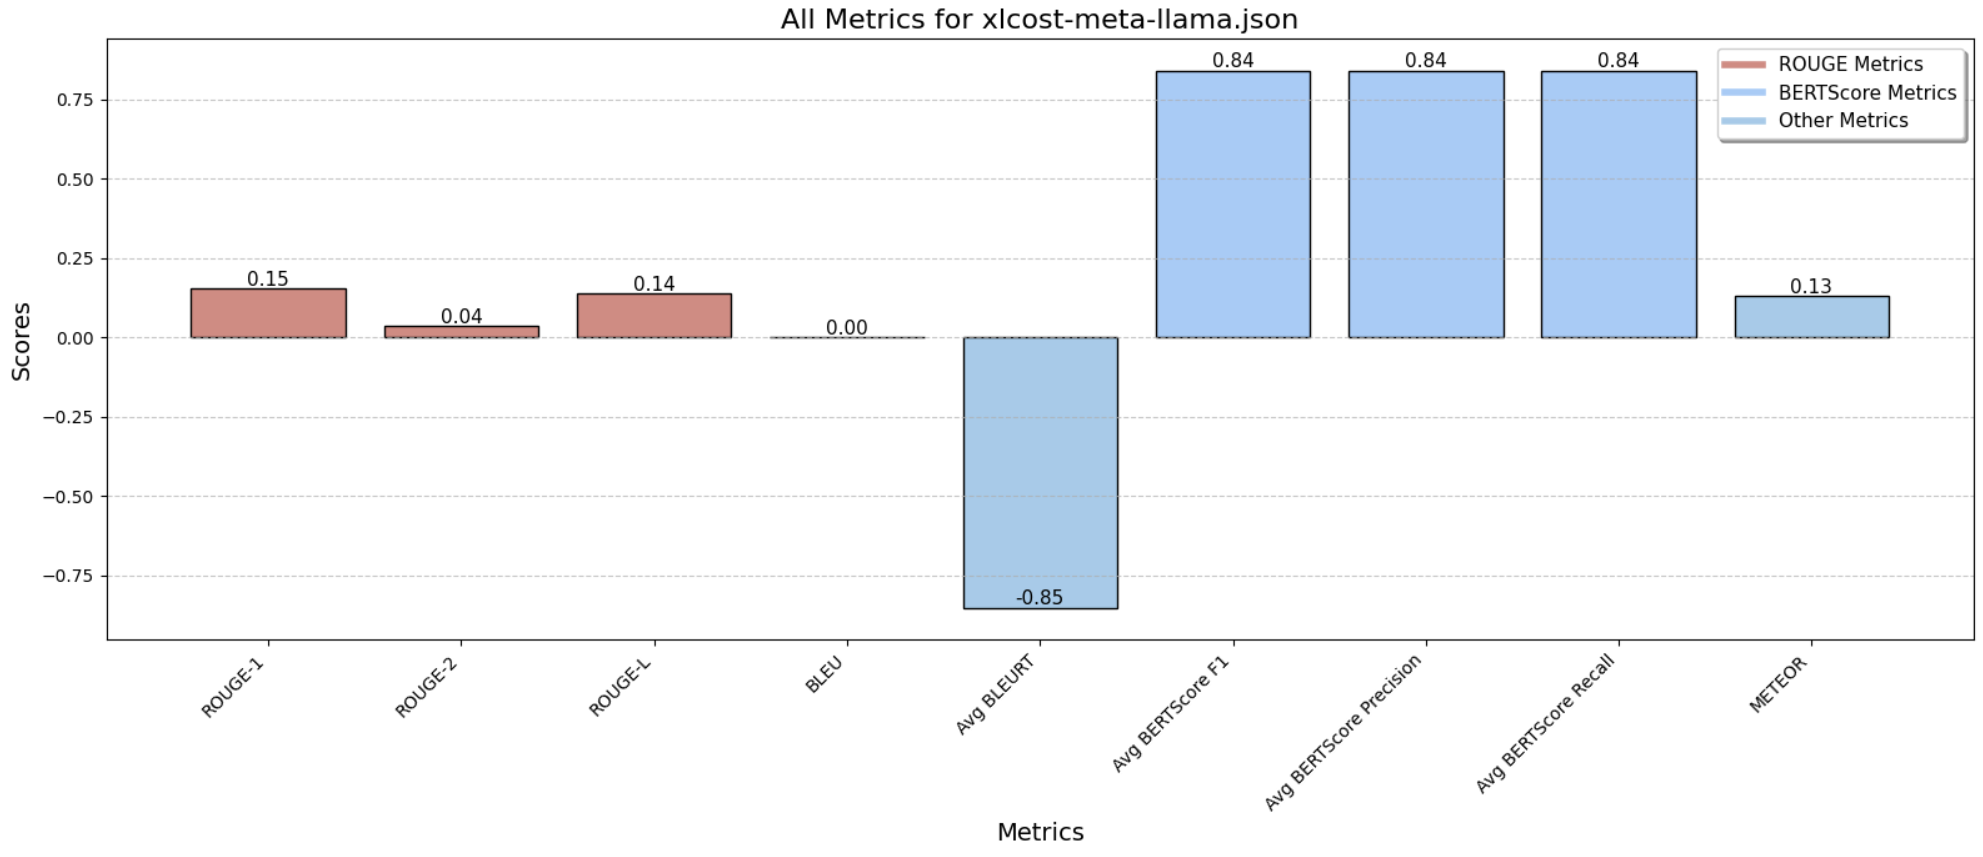
\includegraphics[width=0.8\textwidth]{xlcost-meta-llama.png}
    \caption{Метрики для модели xlcost-meta-llama.json} \cite{github_repo}
    \label{fig:xlcost}
\end{figure}
    
    \vspace{1em}
    
\begin{figure}[H]
    \centering
    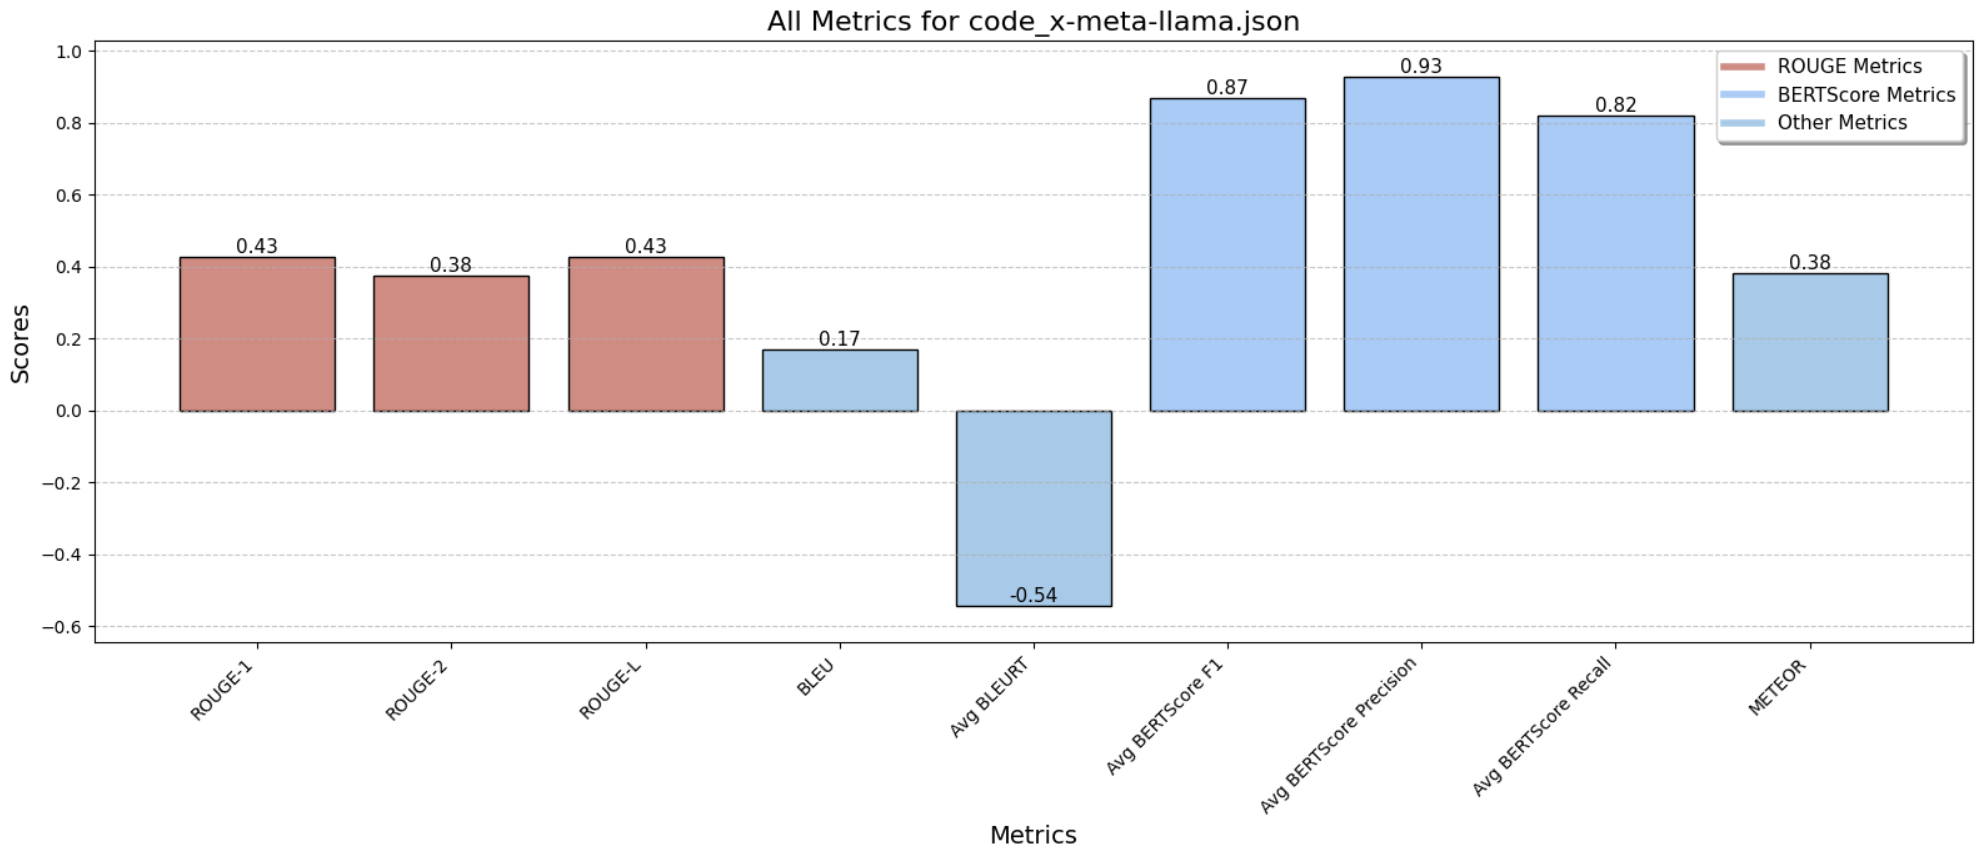
\includegraphics[width=0.8\textwidth]{code_x-meta-llama.png}
    \caption{Метрики для модели xlcost-meta-llama.json} \cite{github_repo}
    \label{fig:code_x}
\end{figure}

    
    \vspace{1em}
\begin{figure}[H]
    \centering
    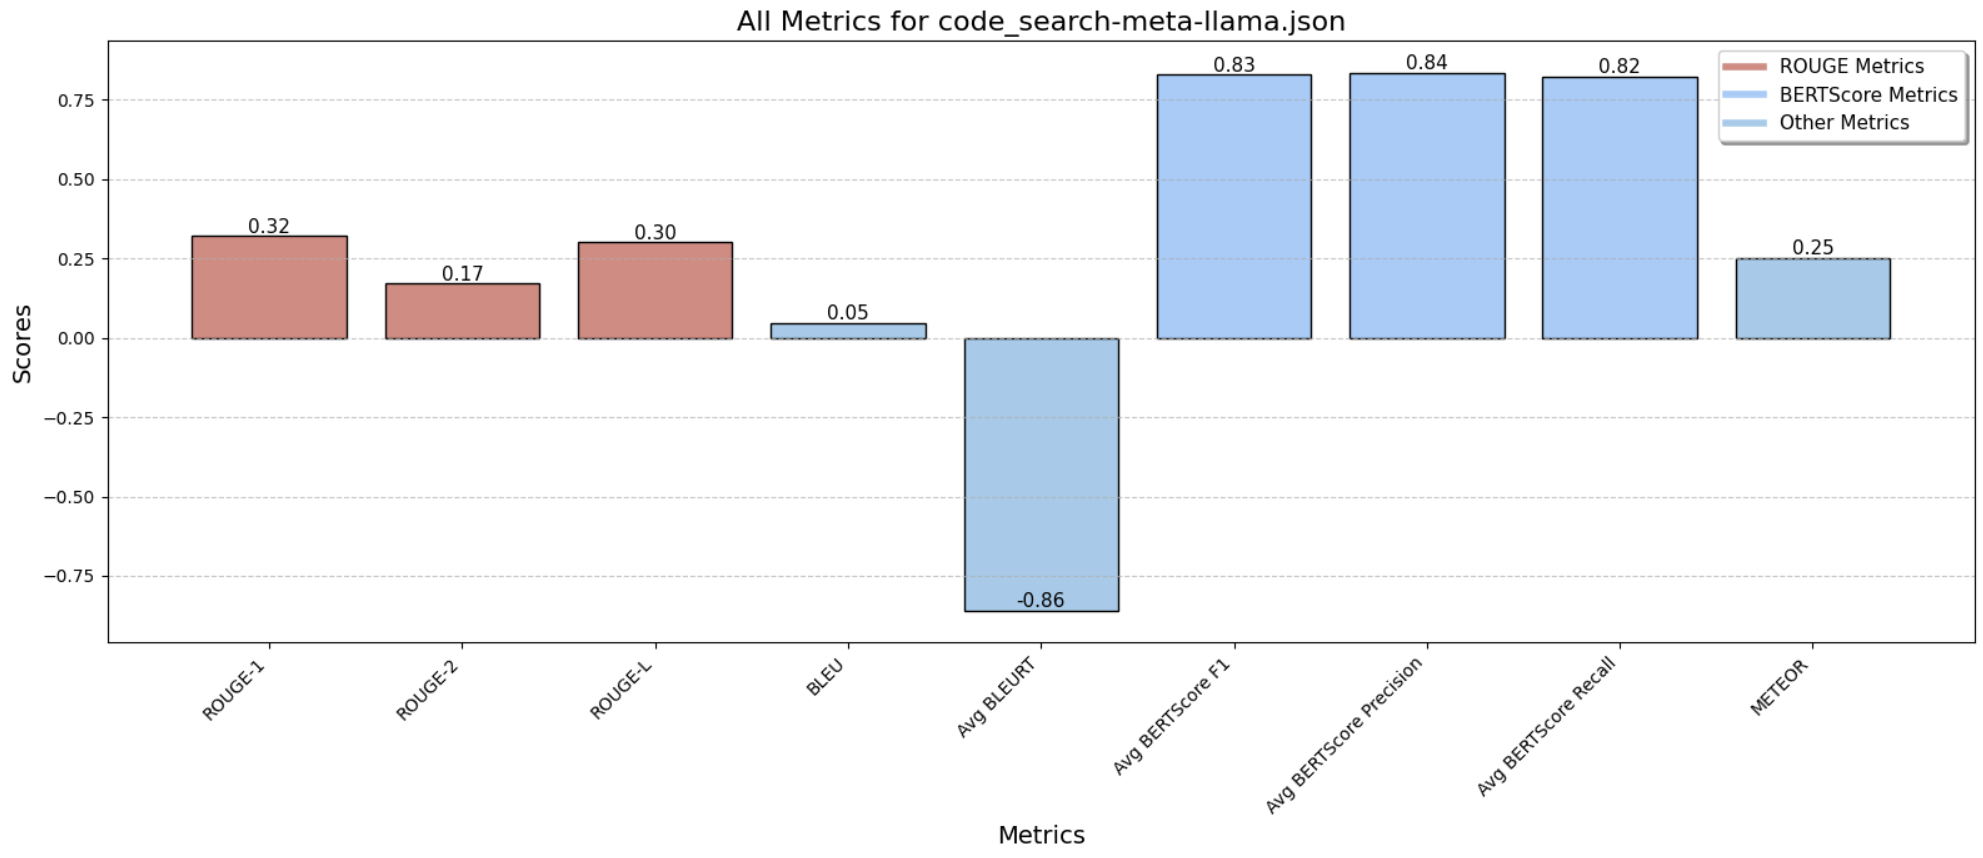
\includegraphics[width=0.8\textwidth]{code_search-meta-llama.png}
    \caption{Метрики для модели xlcost-meta-llama.json} \cite{github_repo}
    \label{fig:code_search}
\end{figure}



\caption{Сравнение метрик для разных моделей}



% Общее описание
На представленных диаграммах (рис.~\ref{fig:xlcost}, \ref{fig:code_x}, \ref{fig:code_search}) видно, что:

    
- Метрики семантического сходства (\textbf{BERTScore}) показывают высокие значения для всех моделей, что указывает на хорошее понимание контекста.
    
- Традиционные метрики (\textbf{ROUGE}, \textbf{BLEU}) дают значительно более низкие оценки, особенно для модели \texttt{xlcost-meta-llama.json} (рис.~\ref{fig:xlcost}), что может быть связано с их чувствительностью к точному совпадению n-грамм.
    
- Отрицательные значения \textbf{Avg BLEURT} для всех моделей свидетельствуют о том, что генерируемые суммаризации воспринимаются как менее естественные по сравнению с эталонными.
    
- Модель \texttt{code\_x-meta-llama.json} (рис.~\ref{fig:code_x}) демонстрирует лучшие результаты по \textbf{ROUGE} и \textbf{BLEU}, что может быть связано с оптимизацией под задачи кодирования.
    
- Разброс значений \textbf{METEOR} (от 0.13 до 0.38) указывает на необходимость дальнейшей настройки метрик для специфичных задач.


Эти данные подтверждают важность использования комбинированных подходов при оценке LLM в контексте кодовой суммаризации.





\newpage
\addcontentsline{toc}{section}{\bf{Список литературы}}
\begin{thebibliography}{99}

% Русскоязычные источники
\bibitem{ahmad2021plbart} 
Ахмад, В.У. PLBART: Pre-trained Model for Programming and Natural Languages / В.У. Ахмад [и др.] // ACL. — 2021.

\bibitem{chen2023} 
Чен, Ю. On the Reliability of Code Summarization Benchmarks / Ю. Чен [и др.] // IEEE Transactions on Software Engineering. — 2023.

\bibitem{feng2023} 
Фенг, М. A Study on BERTScore for Code Summarization / М. Фенг [и др.]. — 2023.

\bibitem{habr2023} 
Статья на Habr: Оценка качества генерации кода. — URL: \url{https://habr.com/ru/articles/745642/} (дата обращения: 15.05.2024).

\bibitem{hu2022lora} 
Ху, И. LoRA: Low-Rank Adaptation of Large Language Models / И. Ху [и др.] // ICLR. — 2022.

\bibitem{karampatsis2020big} 
Карампатсис, Р. Big Code != Good Code: On the Nature of Machine Learning Code / Р. Карампатсис [и др.] // MSR. — 2020.

\bibitem{liu2022survey} 
Лю, Ц. A Survey on Code Intelligence Models / Ц. Лю [и др.] // ACM Computing Surveys. — 2022.

\bibitem{ren2021} 
Рен, С. CodeBLEU: A Method for Evaluating the Quality of Code Summarization / С. Рен [и др.] // Материалы ICSE. — 2021.

\bibitem{wan2023codet5+} 
Ван, И. CodeT5+: Open Code Large Language Models for Code Understanding and Generation / И. Ван [и др.]. — 2023. — arXiv:2305.07922.

\bibitem{wang2021codet5} 
Ван, В. CodeT5: Identifier-aware Unified Pre-trained Encoder-Decoder Models for Code Understanding and Generation / В. Ван [и др.] // EMNLP. — 2021.

\bibitem{zhu2022} 
Чжу, М. XLCoST: A Benchmark Dataset for Cross-Language Code Snippet Transfer / М. Чжу [и др.]. — 2022. — arXiv:2203.04225.

% Англоязычные источники
\bibitem{alon2019code2seq} 
Alon, U. code2seq: Generating Sequences from Structured Representations of Code / U. Alon, S. Levy, E. Yahav // ICLR. — 2019.

\bibitem{austin2021program} 
Austin, J. Program Synthesis with Large Language Models / J. Austin, A. Odena, M. Chen. — 2021. — arXiv:2108.07732.

\bibitem{allamanis2019adverse} 
Allamanis, M. Adverse Results in Program Synthesis: The Case of Neural Code Search / M. Allamanis // Proceedings of the 2019 ACM SIGPLAN International Symposium on New Ideas, New Paradigms, and Reflections on Programming and Software. — 2019. — P. 1–10.

\bibitem{bleurt} 
BLEURT: Evaluating Text Generation with BERT / Google Research. — URL: \url{https://github.com/google-research/bleurt} (accessed: 15.05.2024).

\bibitem{chen2021codex} 
Chen, M. Evaluating Large Language Models Trained on Code / M. Chen [et al.]. — 2021. — arXiv:2107.03374.

\bibitem{codexglue_repo} 
CodeXGLUE Repository / Microsoft. — URL: \url{https://github.com/microsoft/CodeXGLUE} (accessed: 15.05.2024).

\bibitem{codesearchnet_repo} 
CodeSearchNet Repository / GitHub. — URL: \url{https://github.com/github/CodeSearchNet} (accessed: 15.05.2024).

\bibitem{copilot} 
GitHub Copilot: Code Generation Tool / GitHub. — URL: \url{https://github.com/features/copilot} (accessed: 15.05.2024).

\bibitem{feng2020codebert} 
Feng, Z. CodeBERT: A Pre-Trained Model for Programming and Natural Languages / Z. Feng, D. Guo, D. Tang, N. Duan, X. Feng, M. Gong, L. Shou, B. Qin, T. Liu, D. Jiang, M. Zhou. — 2020. — arXiv:2002.08155.

\bibitem{guo2021graphcodebert} 
Guo, D. GraphCodeBERT: Pre-training Code Representations with Data Flow / D. Guo, S. Ren, S. Lu, M. Zhou // Proceedings of the 9th International Conference on Learning Representations. — 2021.

\bibitem{guo2022unixcoder} 
Guo, D. UniXcoder: Unified Cross-Modal Pre-training for Code Representation / D. Guo, S. Ren, S. Lu, M. Zhou // Proceedings of the 44th International Conference on Software Engineering. — 2022. — P. 1418–1429.

\bibitem{husain2019codesearchnet} 
Husain, H. CodeSearchNet: A Benchmark for Code Retrieval and Generation / H. Husain, H. Wu, T. Gazit, M. Allamanis, M. Brockschmidt. — 2019. — arXiv:1909.09436.

\bibitem{lu2021codexglue} 
Lu, S. CodeXGLUE: A Benchmark for Code Understanding and Generation / S. Lu, D. Guo, S. Ren, M. Zhou // Proceedings of the 44th International Conference on Software Engineering. — 2021. — P. 1418–1429.

\bibitem{zaheer2020bigbird} 
Zaheer, M. Big Bird: Transformers for Longer Sequences / M. Zaheer [et al.] // NeurIPS. — 2020.

\bibitem{zhang2020} 
Zhang, T. BERTScore: Evaluating Text Generation with BERT / T. Zhang [et al.]. — 2020. — arXiv:1904.09675.

\bibitem{zhang2020retrieval} 
Zhang, J. Retrieval-based Neural Code Generation / J. Zhang, X. Wang, C. Sun // Proceedings of the AAAI Conference on Artificial Intelligence. — 2020. — Vol. 34(03). — P. 3306–3313.

\bibitem{xlcost_repo} 
XLCoST Repository. — URL: \url{https://github.com/XLCOST/} (accessed: 15.05.2024).

\bibitem{github_repo} 
jachant. Course: репозиторий с метриками оценки LLM для суммаризации кода / jachant // GitHub. — 2023. — URL: \url{https://github.com/jachant/course?tab=readme-ov-file} (дата обращения: 20.10.2023).

\bibitem{zhou2022devign} 
Zhou, Y. Devign: Effective Vulnerability Detection Through Neural Networks / Y. Zhou [et al.] // IEEE S\&P. — 2022.

\end{thebibliography}




\end{document}
